\documentclass[a4paper, 11pt, normalem]{report}

\usepackage{../../../LaTeX-Templates/Notes}
\usepackage{subfiles}
\usepackage{epigraph}

\setlength{\epigraphwidth}{\textwidth}
\titleformat{\part}[display]
{\normalfont\huge\filcenter\bfseries\thispagestyle{epigraph}}
{\partname\ \thepart}
{20pt}
{\Huge}
\titlespacing*{\part}{0pt}{0pt}{40pt}

\title{Atoms, Lasers, and Qubits \vspace{-20pt}}
\author{Dr Weatheril and Prof Adams}
\date{\vspace{-15pt}Michaelmas Term 2019 - Epiphany Term 2020}
\rhead{\hyperlink{page.1}{Contents}}

\begin{document}

\maketitle
\tableofcontents

\epigraphhead[200]{\hfil\includegraphics{lasers.png}\hfil}
\part{}
\chapter{}
\begin{itemize}
    \item \textbf{Note:} The course will be more reading based than math based. 
Read the references on each summary sheet. 
    \item Need light oscillation, not just amplification.  
    \item 1 in $10^{18}$ atomic clock accuracy.
    \item LD: laser diode
    \item Non-linear crystals allow different wavelengths
    \item Laser transitions based on E group of materials
    \item Learn the unit conversions
    \item Magneto-optical trap to cool atoms
    \item Optical frequency comb $\to$ accurate measurement of wavelength of light 
    \item Sodium atoms in upper atmosphere which we fluoresce for AO
    \item \textbf{LEARN!} Q on paper always - contents of a laser
        \begin{enumerate}
            \item More in excited state than ground
            \item Pump gets energy in
            \item Mirrors to make light bounce back and forward
        \end{enumerate}
\end{itemize}

\section{Introduction to lasers}
Lasers - coherence $\to$ 2 types - longitudinal and transverse
\begin{itemize}
    \item Lasers are highly coherent, both transversely and longitudinally. 
        Longitudinal and temporal coherence is related to linewidth, and will be discussed. 
        Coherence length $l_c$ and coherence time $\tau_c$ are the distance and time over which a coherent wave maintains a specified degree of coherence, i.e. when its phase is predictable. 
\end{itemize}
\begin{multicols}{2}
\begin{figure}[H]
    \centering
    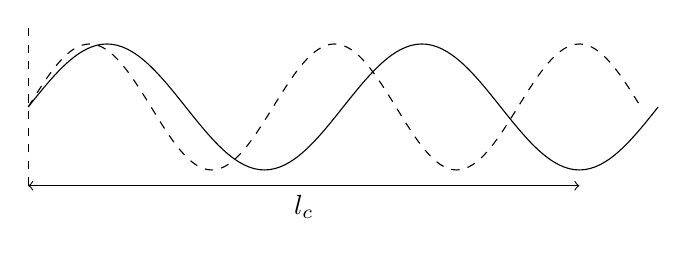
\begin{tikzpicture}
        \draw[dashed] (0,0) -- (0,2);
        \draw[<->] (0,0) -- (7,0) node[anchor=north,midway] {$l_c$};
        \draw (0,1) sin (1,1.8) cos (2,1) sin (3,0.2) cos (4,1) sin (5,1.8) cos (6,1) sin (7,0.2) cos (8,1);
        \draw[dashed] (0,1) sin (0.78,1.8) cos (1.56,1) sin (2.33,0.2) cos (3.11,1) sin (3.89,1.8) cos (4.67,1) sin (5.44,0.2) cos (6.22,1) sin (7,1.8) cos (7.78,1);
    \end{tikzpicture}
\end{figure}
\columnbreak
Coherence length and time:
\begin{align}
    l_c &= \frac{2\pi c}{\delta\om},~~  \tau_c = \frac{2\pi}{\delta\om}
\end{align}
\end{multicols}
\begin{itemize}
    \item Can't have an infinitely narrow spectrum. 
        Monochromaticity - laser has a spectral linewidth $\delta\om$, this is much smaller than the actual carrier/centre frequency. $\delta\om\ll\om_0$ for a laser where $\om_0$ is the centre frequency. 
        From mHz to GHz in range. 
    \item Highly directional beam $\to$ energy contained in one region. 
\end{itemize}
Directionality:
\begin{itemize}
    \item Lasers have highly directional beams that diverge due to diffraction
    \item Beam will be larger
    \item Waist of beam, $2\om_0$.
\end{itemize}
\begin{figure}[H]
    \centering
    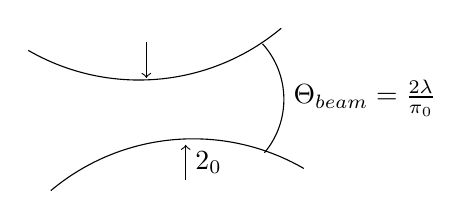
\begin{tikzpicture}
        \draw (0,1) arc (240:310:80pt);
        \draw (3.5,-0.5) arc (60:130:80pt);
        \draw (3,-0.3) arc (-40:42:30pt) node[anchor=west,midway] {$\Theta_{beam} = \frac{2\lambda}{\pi\om_0}$};
        \draw[->] (1.5,1.1) -- (1.5,0.65);
        \draw[->] (2,-0.65) -- (2,-0.2) node[anchor=west,midway] {$2\om_0$};
    \end{tikzpicture}
\end{figure}
\begin{itemize}
    \item All in a very low frequency range $\to$ all energy oscillating in small aarea in small frequency range - useful applications. 
\end{itemize}
Brightness:
\begin{itemize}
    \item Lasers are spectrally bright
    \item Definition of brightness - amount of power in particular area (solid angle) of the beam:
        \begin{equation}
            B_\om = \frac{P}{A\Delta\Om\Delta\om},
        \end{equation}
        where $A$ is the area, $\Delta\Om$ is the solid angle, and $\Delta\om$ is the linewidth. 
\end{itemize}
Electromagnetic Field Modes - not examinable:
\begin{itemize}
    \item 1st Chapter of 'Laser Physics' book
    \item Planck's radiation law
    \item Each unique solution of field is EM mode
    \item $L^3$ factored out when divided by volume
    \item Modes exist with or without energy
\end{itemize}


\end{document}
















